\section{(1.5)}

We are looking at the wave function

\begin{equation}
    \Psi(x,t) = Ae^{-\lambda\abs{x}}e^{-i\omega t}
\end{equation}

\begin{parts}
    \item To normalize, we can choose $t=0$, though it really doesn't matter since the modulus square will eliminate the time-dependence anyways:
        \begin{equation*}
            A^2 \intinf e^{-2\lambda\abs{x}} \;\dd x = 1.
        \end{equation*}
        The fact that there is an absolute value around the $x$ in the exponential makes the integrand even, so we can change the limits, add a factor of 2, and remove the absolute value:
        \begin{gather*}
            2A^2 \int_0^{\infty} e^{-2\lambda x} \;\dd x = 1, \\
            2A^2 \cdot -\frac{1}{2\lambda} \left[e^{-2\lambda x}\right]^{\infty}_0 = 1, \\
            A^2 \cdot \frac{1}{\lambda} = 1, \\
            \boxed{A = \sqrt{\lambda}.}
        \end{gather*}
    \item We can just use the definition of expectation value:
        \begin{equation*}
            \braket{x} = \intinf \psi^* x \psi \;\dd x = \lambda \intinf x e^{-2\lambda \abs{x}} \;\dd x.
        \end{equation*}
        Here, $x$ is an odd function, and, as established in part (a), the exponential is an even function. The product of an odd and even function is an odd function, and since we are evaluating it over a symmetric interval, it is zero:
        \begin{equation*}
            \boxed{\braket{x} = 0.}
        \end{equation*}
        Next,
        \begin{equation*}
            \braket{x^2} = \lambda \intinf x^2 e^{-2\lambda\abs{x}} \;\dd x = 2\lambda \int_{0}^{\infty} x^2 e^{-2\lambda x} \;\dd x.
        \end{equation*}
        From the integral table, we have that
        \begin{equation}
            \int_0^{\infty} x^n e^{-x/a} \;\dd x = n! a^{n+1}.
        \end{equation}
        Here, we have that $n=2$ and $a = 1/2\lambda$, so our integral becomes:
        \begin{equation*}
            \braket{x^2} = 2\lambda \cdot 2! \left(\frac{1}{2\lambda}\right)^3 = \boxed{\frac{1}{2\lambda^2}.}
        \end{equation*}
    \item The standard deviation is
        \begin{equation}
            \sigma_x = \sqrt{\braket{x^2} - \braket{x}^2} = \sqrt{\frac{1}{2\lambda^2}} = \boxed{\frac{\sqrt{2}}{2\lambda}.}
        \end{equation}
        \begin{figure}[ht]
            \centering
            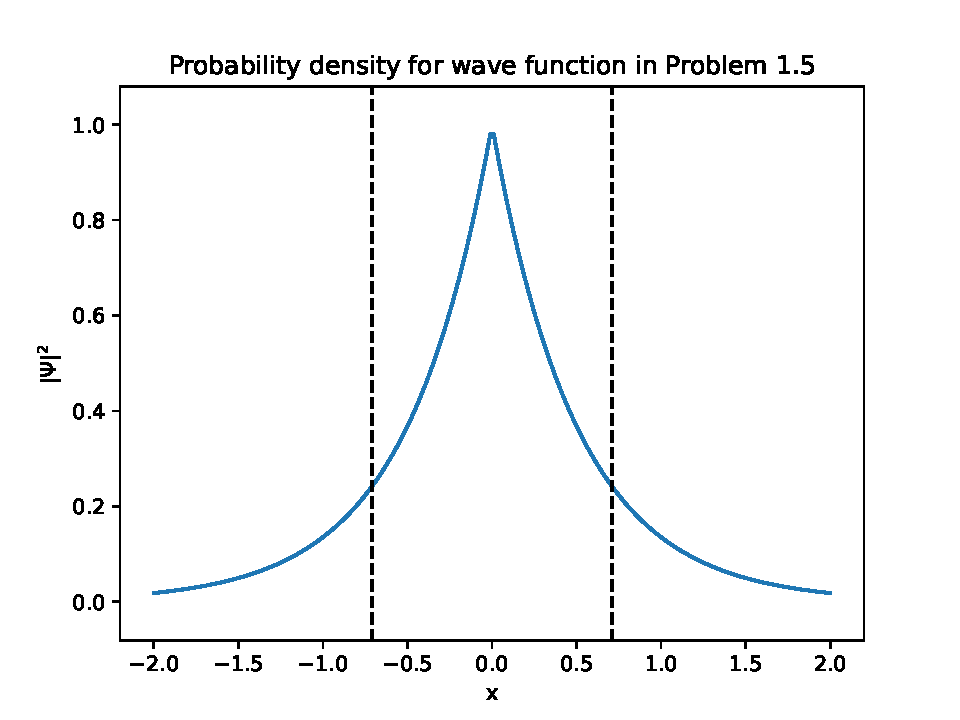
\includegraphics[scale=0.7]{./res/plot.pdf}
            \caption{The $\abs{\Psi}^2$ distribution with the standard deviations marked with black dotted lines.}
            \label{PartDPlot}
        \end{figure}
        A plot of the $\abs{\Psi}^2$ distribution is given in Figure~\ref{PartDPlot}, where the vertical black lines are $x = \braket{x} - \sigma_x$ and $x=\braket{x} + \sigma_x$. To determine the probability that a particle lies outside this range, we integrate over the whole space, excluding the bit inside. Again exploiting the fact that our integrand $\abs{\Psi}^2$ is even, we can look at just the upper half, say, which is
        \begin{align*}
            P(x \notin [-\sigma_x, \sigma_x]) &= 2 \lambda \int_{\sigma_x}^{\infty} e^{-2\lambda x} \;\dd x, \\
            &= -1 \left[e^{-2 \lambda x}\right]_{\sigma_x}^{\infty}, \\
            &= e^{-2\lambda \cdot \sqrt{2}/2\lambda^2} = e^{-\sqrt{2}}, \\
            \Aboxed{P(x \notin [-\sigma_x, \sigma_x]) &= e^{-\sqrt{2}} \approx 0.243.}
        \end{align*}
\end{parts}